\chapter{实验分析与讨论}
本章将详细描述本文所使用的数据集,实验设计以及对于实验结果的评价标准。本文在第三章提出了
在网络表征算法HLE及其增量表征算法iHLE,第四章中提出了在属性网络中的表征算法SR及其增量网络场景下的表征算法iSR,本章将在数据集上进行相关的实验并与其他著名算法进行对比分析。

%%%%%%%%%%%%%%%%%%%%%%%%%%%%%%%%%%%%%%%
%----------------------------------------     数据介绍     ---------------------------------------%
%%%%%%%%%%%%%%%%%%%%%%%%%%%%%%%%%%%%%%%
\section{数据介绍}
本文利用的数据集为5个真实数据集,其中真实数据集包括2个社交媒体数据和3个引用网络数据。这5个数据集都是在线公开数据\footnote{https://linqs.soe.ucsc.edu/data}\footnote{people.tamu.edu/~xhuang/Code.html}
\begin{itemize}
	\item \textbf{BlogCatalog}: BlogCatalog是一个社交媒体网站,用户在上面发表博客并通过相互关注建立网络,数据集选取了5196个用户节点,包含了171,743条连边。用户节点的属性信息来自用户博客的关键词描述加工处理而成,构建了8189维用户节点的属性特征,用户的分类标签是从用户自定义的兴趣爱好中选择得来的。
	
	\item \textbf{Flickr}:Flickr是一个图片分享社区,用户通过图片分享与其他用户交互,数据集以用户间的相互关注组成网络,数据集选取了7575个用户节点,包含了239,728条连边,用户节点的属性信息来源于用户的分享内容的标签(tag)信息,提取了12047维节点属性特征。用户的分类信息来源用用户加入的兴趣社区。
	
	\item \textbf{Citeseer}:Citeseer数据集是从挑选Citeseer网站上的一些文献,文献的选择过程保证对于每一篇文献都有至少被一篇文献所引用,总共选取了3312篇文章作为网络中的节点,构建了一个文献引用网络。文献的属性是来自对内容的处理得到,通过去掉停用词和选取词干的方法,剩下的3703个单词组成词库,在对文献进行处理的时候,出现次数小于10的单词去掉,根据文献中是否存在词库对应单词,将对应特征置为0/1,于是文献节点属性特征维数为3703维。根据文献本身所属主题,文献被分为六个类别:Agents,AI,DB,IR,ML和HCI。
	
	\item \textbf{Cora}:Cora是另一个论文引用网络,主要是机器学习细分领域的论文之间的引用关系,同样在构造数据集的时候保证最后每一篇论文都有至少有一个被引用量,该数据集包含2708篇论文,在提取论文节点的属性特征时,采用方法跟Citeseer类似,通过对全部文献去掉停用词、处理词干构建词库,去掉每篇文章中的出现少10次的词,得到1433维属性特征。根据论文的内容,将论文节点分成6种:Case Based, Genetic Algorithms, Neural和Networks, Probabilistic Methods, Reinforcement Learning, Rule learning和 Theory。
	
	\item \textbf{PubMed}: PubMed是另一个论文引用网络,主要涉及的是生物领域的文献。数据集选取了19717个论文作为网络节点,不同的是,论文节点的属性特征不是0/1型,而是用文档中对应单词TF-IDF加权得到。数据集中论文根据研究主题被分成3类:Diabetes Mellitus Experimental,Diabetes Mellitus Type 1和Diabetes Mellitus Type 2。
	
\end{itemize}
关于上述数据的具体详情,见下表,另给出BlogCatalog数据集中的度分布情况。
\begin{table}
\centering
\caption{使用数据集详细统计信息}
\begin{tabular}{C{1in}C{1in}C{1in}C{1in}C{1in}}
\textbf{数据集} & \textbf{节点数} &\textbf{连边数} & \textbf{属性数}&\textbf{类别数}\\ \hline 
BlogCatalog & 5186  & 171,743 &8189&6\\
Flickr	& 7575 &239,728 & 12,047 & 9 \\
Citeseer& 3312 & 4536  &  3703 & 6 \\
Cora & 2708 &5429 & 1433 &7 \\
PubMed & 19,717 &44,338&500 &3 \\
\hline
\end{tabular}
\end{table}

\begin{figure}
	\centering
	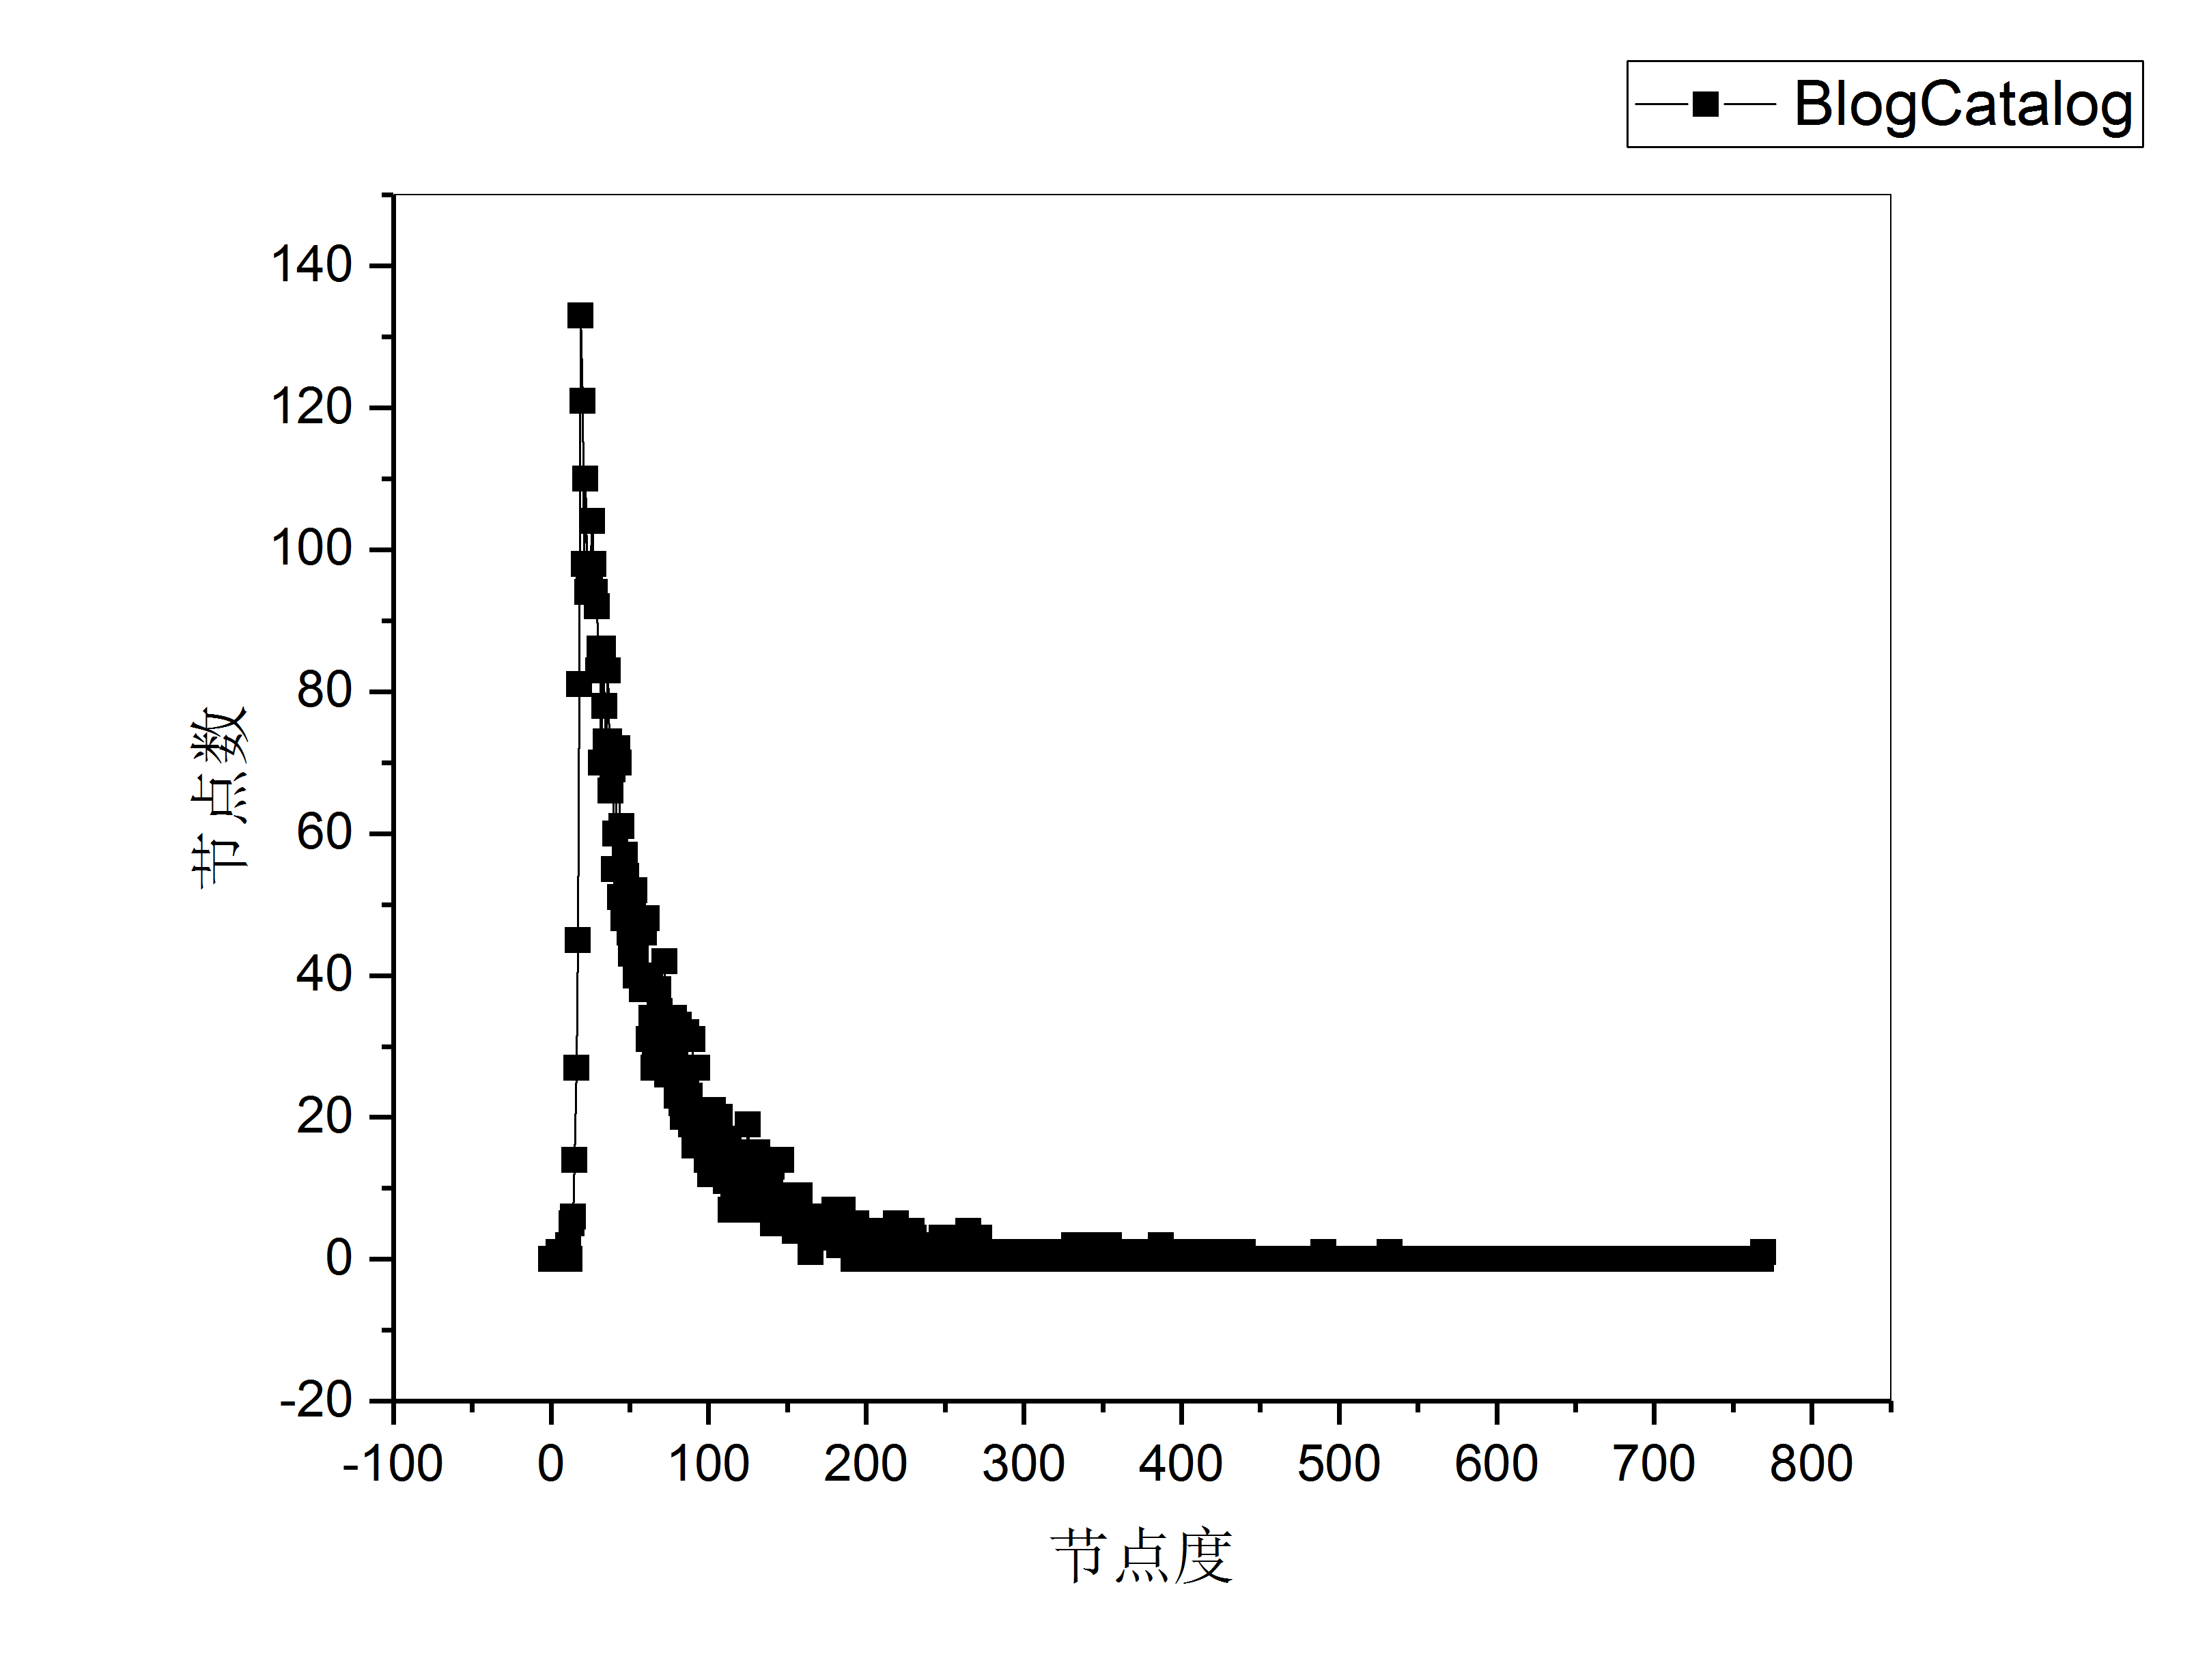
\includegraphics[width=5in]{figures/blogCatalog_degree}
	\caption{案例数据:BlogCatalog中的度分布}
\end{figure}
\section{实验环境}

\section{实验设计}
图表征算法是对网络中节点进行向量表征的过程,在这一部分主要从两方面对前面章节提出的算法进行分析评价:
\begin{itemize}
	\item \textbf{准确性}:图表征算法学习到的向量表征需要应用于后续的机器学习任务,在不同的机器学习任务中表现出来的分类预测效果如何,跟其他算法的对比效果如何?
	\item \textbf{运行效率}:基于动态增量场景提出的算法运行效率如何,跟其他离线批量算法在效率上的差异。
\end{itemize}
本节将分别从这两方面提出设计的实验过程。
\subsection{准确性评估}
在准确性评估这一部分,本章主要针对两个学习任务来进行具体的对比:一个是节点多分类任务,一个是图挖掘中常见的链路预测问题。对于不同的学习任务有不同的实验设计过程和评价准则,下面将分别对这些实验的具体过程进行介绍。

\problem{\textbf{节点多分类实验}:}节点多分类问题在一个监督学习任务,在对节点进行向量表征之后需要划分训练集和测试集,通过训练集训练模型,对测试集中的数据进行预测并评估结果的好坏。分类问题的评估方法有很多,不同于普通的二分类问题,节点分类问题是多分类过程,在节点分类任务中一般采用的评测指标有三种:分类准确率(accuracy), F1-Macro和F1-Micro。

{\textbf{衡量指标1:分类准确率}} :准确率的定义是对于给定的测试样本集,分类模型预测类别正确的样本占总样本的比例,从损失函数的角度来讲,就是模型损失函数为0-1阶梯函数时测试集上的损失值。

{\textbf{衡量指标2:F1-Macro和F1-Micro}}在介绍这两个评价准则之前,需要介绍F1值。在二分类问题中,根据实际的类别标签和预测的类别标签的不同情况可以得到混淆矩阵:
\begin{table}
	\centering
	\caption{混淆矩阵}
	\begin{tabular}{|c|c|c|c|}
		\hline
		\multirow{2}*{预测标签}& \multicolumn{2}{|c|}{真实标签} \\
		\cline{2-3}
		~ & 正例 & 反例 \\ \hline
		正例 & TP(真正例) & FP(假正例) \\ \hline
		反例 & FN(假反例) & TN(真反例) \\
		\hline
	\end{tabular}
\end{table}

其中精度P(Precision)和召回率R(Recall)可以根据混淆矩阵定义出来:
\begin{equation}
\begin{aligned}
P &= \frac{\#TP}{\#TP+\#FP} \\
R &= \frac{\#TP}{\#TP+\#FN}
\end{aligned}
\end{equation}
其中$\#\cdot$表示对应样本的个数,考虑在现实场景中精度和召回率各有不足,召回率偏向于将样本都预测为正样本,精度需要保证预测中真实正样本的比例,会偏向于将预测正样本的个数降低,F1值综合考虑精度和召回率,对两者进行统一:
\begin{equation}
	F1 = \frac{2\times P\times R}{P+R}
\end{equation}
可以看出$F1$为精度和召回率的调和平均。

在多分类问题中,无法通过二元的混淆矩阵来表示样本预测与真实之间的关系,对于$F1$因此有了在多分类情况的变形F1-macro和F1-micro。在多分类场景下需要将不同类别两两之间计算混淆矩阵,算出对应的精度和召回率,F1-macro的计算方法是:
\begin{equation}
	macro\-P = \frac{1}{n}\sum P_i
\end{equation}
\begin{equation}
macroR = \frac{1}{n}\sum R_i
\end{equation}
\begin{equation}
F1macro = \frac{2\times macroP\times macroR}{macroP+macroR}
\end{equation}
在计算完混淆矩阵后,对所有矩阵的对应值去平均得到$\overline{TP}, \overline{TN}, \overline{FN},\overline{FP}$,可以得到F1-micro的计算方法:
\begin{equation}
microP = \frac{\overline{TP}}{\overline{TP}+\overline{FP}}
\end{equation}
\begin{equation}
microR = \frac{\overline{TP}}{\overline{TP}+\overline{FN}}
\end{equation}
\begin{equation}
F1micro = \frac{2\times microP\times microR}{microP+microR}
\end{equation}
对于节点多分类问题,本章对所有数据集进行比例抽样,从10\%到100\%对数据进行抽样,进行embedding后,进行节点多分类任务,多分类学习任务采用逻辑斯蒂回归(Logistic Regression)算法进行学习,数据集通过5折交叉进行多次训练验证,并通过准确率,F1-macro,F1-micro三个指标对算法效果进行评估。在对算法进行准确性评判时,分成两个部分:\textbf{离线模型}和\textbf{在线模型}。对于\textbf{离线模型}跟已有的图表征算法的效果进行对比:
\begin{itemize}
	\item 拉普拉斯特征映射算法LE:基于保留一阶接近度的图表征方法,将问题转化为求矩阵特征值的问题
	\item LINE算法:通过保留一阶接近度和二阶接近度进行图表征的算法,通过负采样优化计算。
	\item Node2vec算法:借用自然语言处理中的Word2vec思想,通过随机游走生成节点语料库,从而对图进行表征学习。
	\item CCA算法\cite{hardoon2004canonical}:将原始网络结构和原始属性特征直接作为节点分类任务的输入。
	\item AANE算法\cite{huang2017label}\footnote{https://github.com/xhuang31/AANE\_python}:将网络结构特征和属性特征同时进行优化,得到属性网络表征作为后续学习任务的输入。
	\item HLE算法:本文提出的基于高阶接近度的拉普拉斯特征映射算法。
	\item SR算法:本文提出的基于属性相似度的表征算法。
\end{itemize}
通过下面的表对实验中采用的算法进行分类:
\begin{table}
	\centering
	\caption{节点分类任务图表征算法分类}
	\begin{tabular}{|C{2in}|C{3in}|}
		\hline
		\textbf{类别} & \textbf{算法} \\ \hline 
		\multirow{4}*{网络表征}&拉普拉斯映射算法LE \\ 
		\cline{2-2}
		~ &  LINE算法	\\ 	\cline{2-2}
		~ &	 Node2Vec算法 \\ \cline{2-2}
		~ &  HLE算法	\\ \hline
		属性表征 & SR算法 \\ \hline
		\multirow{3}*{属性网络表征} & CCA算法 \\ \cline{2-2}
		~ & AANE算法 \\ \cline{2-2}
		~ & HLE+SR算法 \\ \hline
	\end{tabular}
\end{table}

\textbf{在线模型}的准确性评估实验不同于离线模型的实验设计。在离线模型评估中采用的方式为随机按比例抽样进行学习任务,不同比例的样本不存在包含关系。而在线模型中将样本分成不同的时间步,依次加入网络中进行,因此后一个时间步包含前一个时间步的样本整体。在这里需要注意的一点是,在实验过程中抽样过程先于表征算法,先完成抽样再进行表征学习,在节点分类任务时存在的训练测试集分割则在表征算法之后进行。对于在线模型,实验过程主要跟对应的离线进行准确性对比。

在对图表征算法进行准确性评判,本文还将表征向量应用于链路预测实验。
\problem{\textbf{链路预测问题}}:链路预测问题也是一个监督学习任务,但是不同于节点多分类任务的标签来源于其他附加信息,链路预测问题的标签来源于网络中的连边。链路预测问题的初衷是根据网络结构中已经存在的连边,预测没有产生连接的节点对中产生连接的概率,链路预测问题原本是基于网络对网络的学习,进一步扩展在属性网络中,利用节点本身的属性特征提高预测效果。

\textbf{属性网络中的链路预测}:给定无向属性网络$G(V,E,H)$,其中$V$代表节点集合,$E$代表连边的集合,$H$代表网络节点的属性特征集合,根据节点集合可以算出网络中所有可能连边的集合为$U$,集合的大小为$|U| = \frac{|V|(|V|-1)}{2}$,链路预测问题就是需要通过一定的算法对连边$E\prime\in U\setminus E$的可能性进行预测,也即对不存在(或未被观测到)的连边预测存在的概率。

在传统的监督学习任务中每条样本对应有特征和一个(或多个)类别标签,在模型训练之前划分训练集和测试集。本文中的链路预测也需要进行训练集和测试集的划分,在训练集中需要包含正样本和负样本,测试集也同样需要包含正负样本,正样本为在网络中确实存在的连边,也即$E$中连边,负样本连边来源于$U\setminus E$,关于训练集和测试集的划分过程如下图:
\begin{figure}
	\centering
	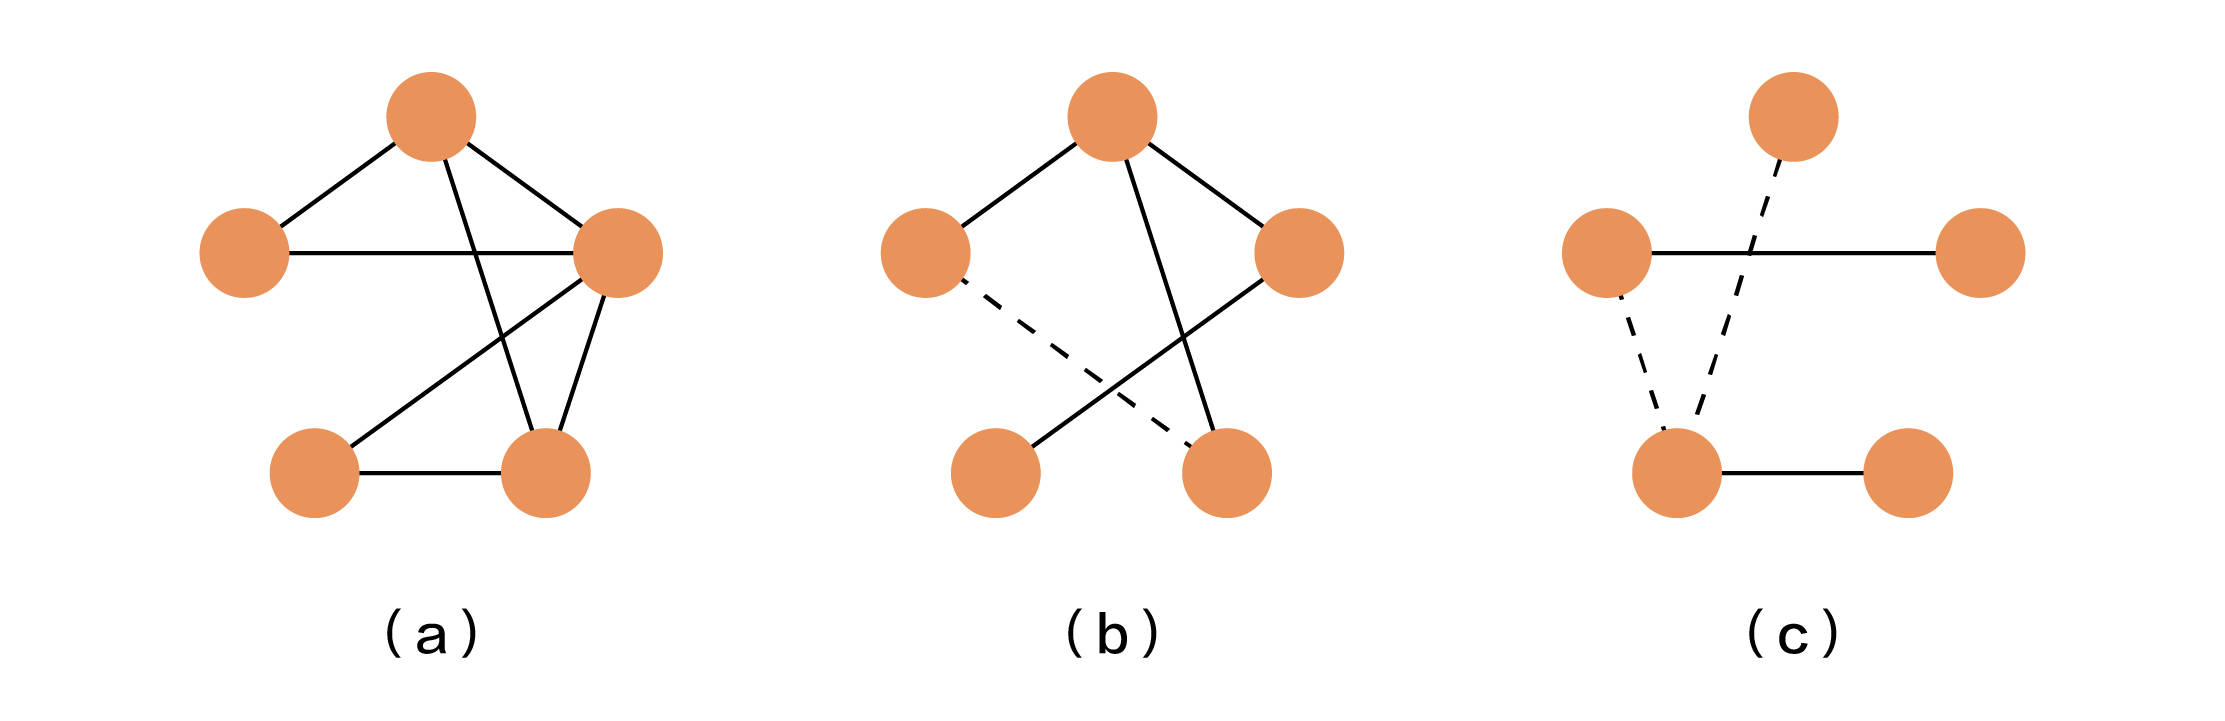
\includegraphics[width=6in]{figures/link_prediction_split}
	\caption{链路预测训练测试集划分:(a)全部连边$E$;\\(b)训练集:包含正负样本,负样本用虚线表示(c)测试集:包含正负样本}
\end{figure}

不同于上面的节点分类任务,在链路预测实验中不是直接针对节点进行k折交叉验证实验,链路预测的训练测试集是针对连边进行采样得到的,图表征算法学习到的是节点的向量表征,将图表征用于链路预测任务的直观方法是,将关于连边$e$的节点对$(i,j)$的表征向量$X_i,X_j$的函数$f(X_i, X_j)$作为该连边$e$的特征,在本文实验中采用$f(X_i, X_j) = X_i\circ X_j$ ,也即$X_i, X_j$对应元素相乘作为边的特征,再放入二分类的学习算法中,在实验中本文采用的分类算法是逻辑斯蒂回归(Logistic Regression),实验效果在测试集上进行通过\textbf{AUC}和\textbf{准确率}进行效果评价,准确率之前提及过,下面介绍一下AUC评价标准。

\textbf{衡量指标1:AUC}:AUC(Area under ROC curve),意思就是ROC(Receiver Operating Characteristic)曲线下的面积,ROC曲线是以真正例率(True Positive Rate,简称TPR)和假正例率(False Positive Rate, FPR)画出的曲线,其中以FPR为横轴,TPR为纵轴,根据混淆矩阵中的定义有:
\begin{equation}
	TPR = \frac{\#TP}{\#TP+\#FN}
\end{equation}
\begin{equation}
FPR = \frac{\#FP}{\#TN+\#FP}
\end{equation}
ROC曲线将样本按照预测概率从大到小排序,从第一个样本依次设置分类阈值为其预测值,并以此对所有样本判定预测的正负值,进一步计算出一组TPR和FPR值,以此循环可以得到一系列的值形成ROC曲线,AUC则是ROC曲线下的面积,AUC评价方法关注的是预测样本概率的排序质量。同样的,在这一部分增量学习算法主要跟对应的离线算法进行准确性对比链路预测的实验过程如下图所示:
\begin{figure}
	\centering
	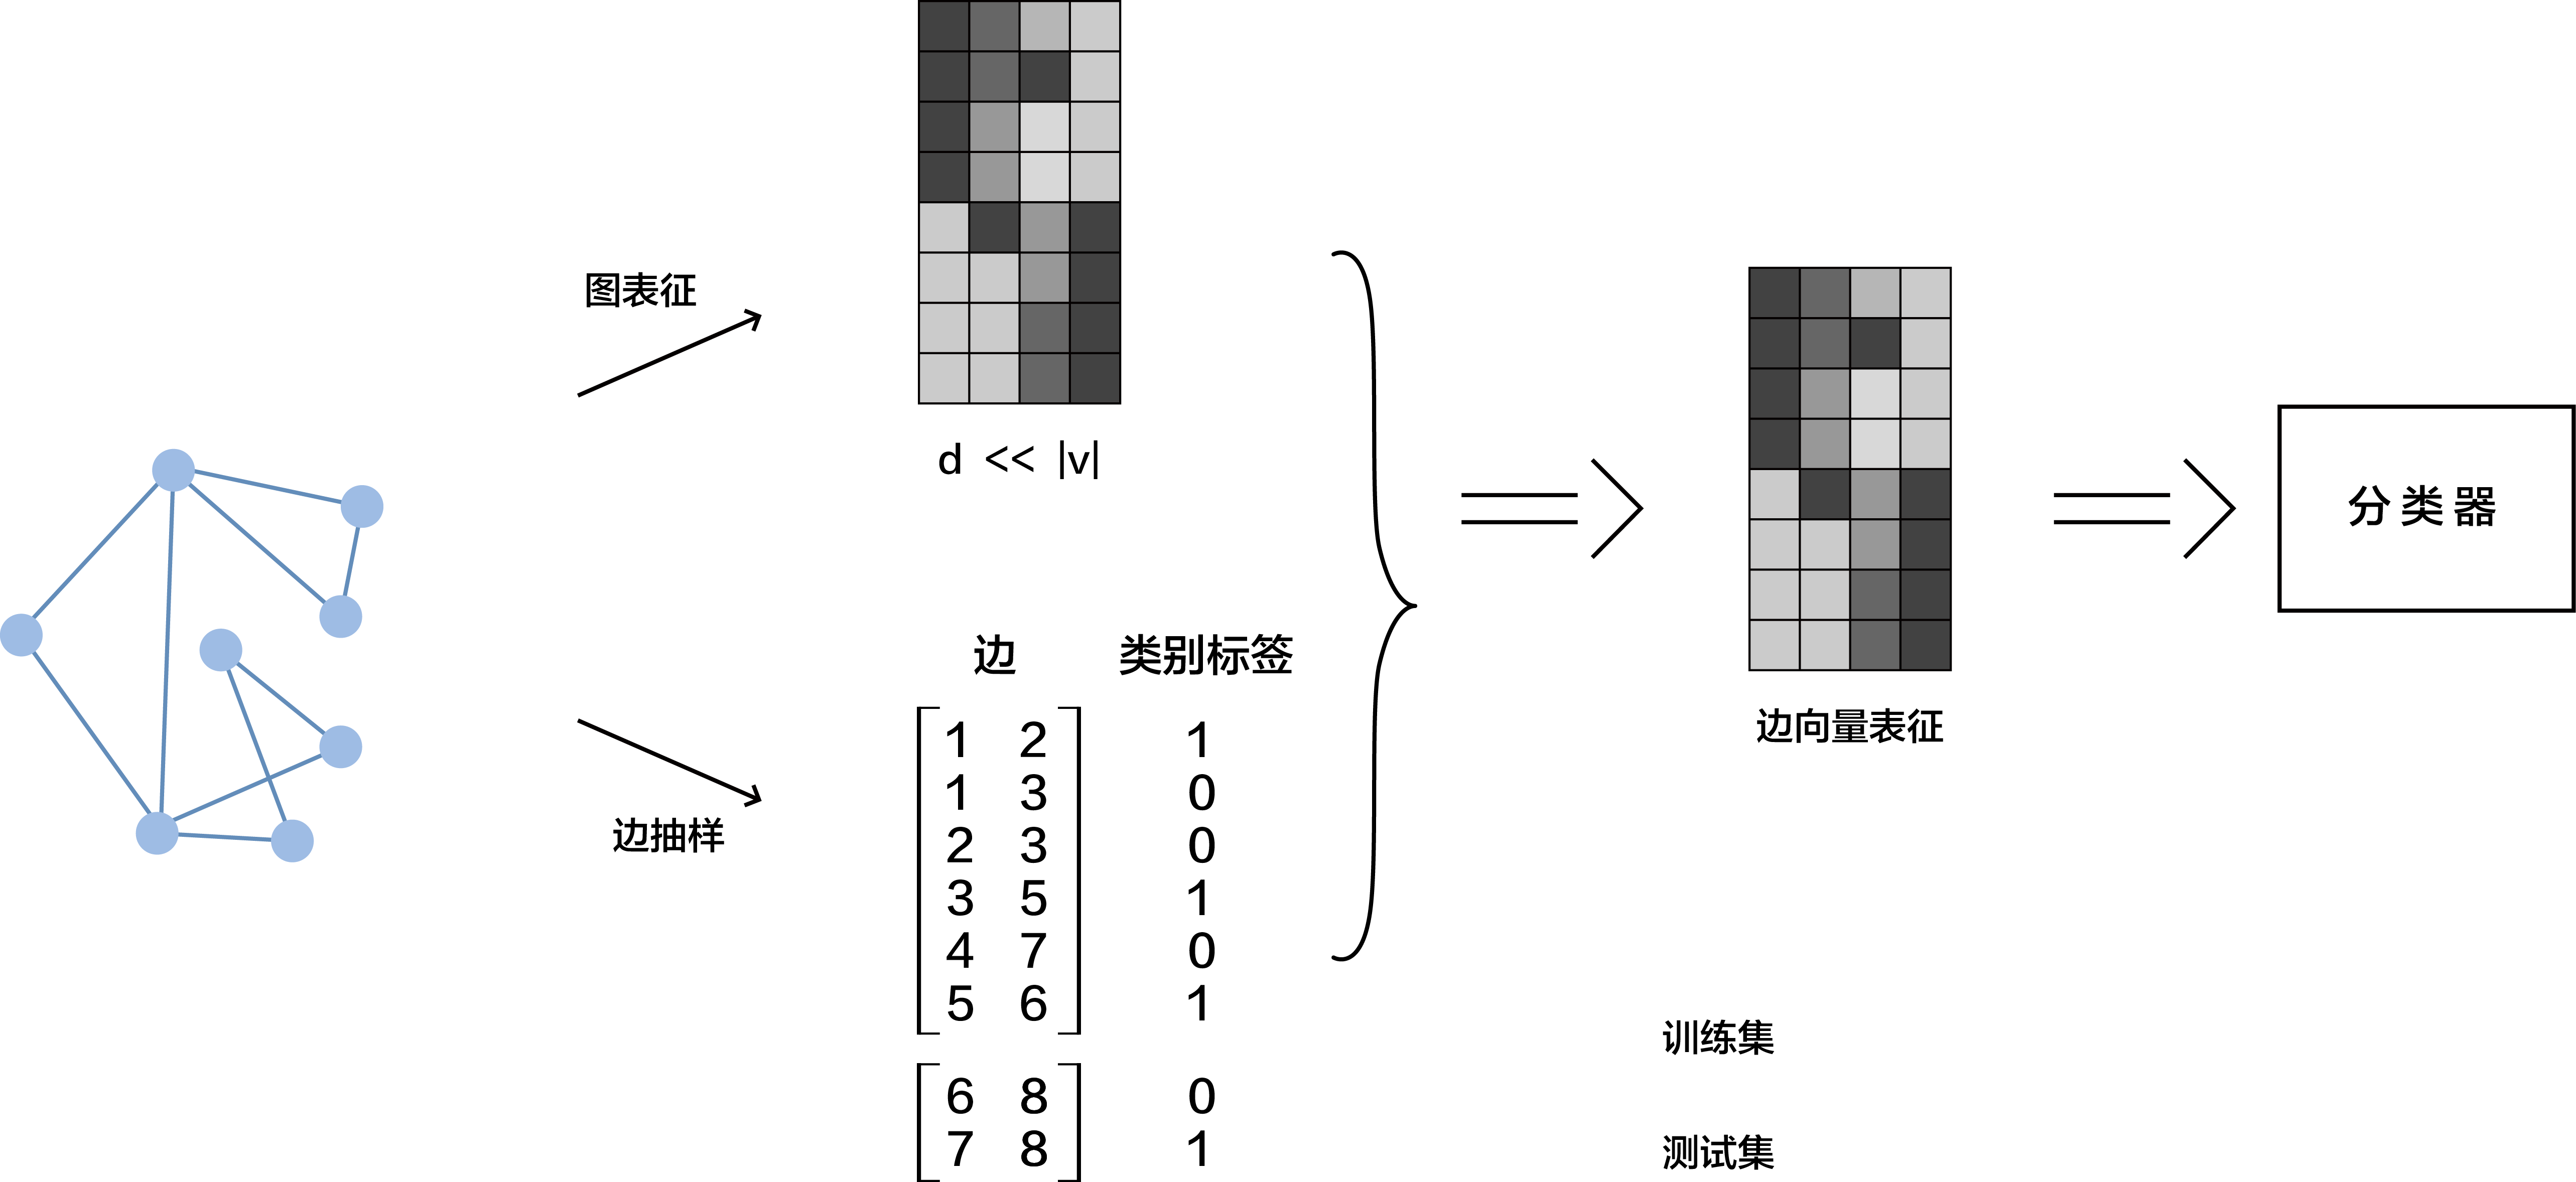
\includegraphics[width=6in]{figures/link_predict_frame}
	\caption{链路预测实验过程}
\end{figure}

\subsection{运行效率评估}
在运行效率评估这一部分,主要进行增量算法跟离线算法之间的对比,将数据集分解成多个时间步,在最初的时间步采用离线算法进行图表征,在第二个及以后时间步将分成增量算法和离线算法进行表征学习,并从两方面来对算法效果进行对比评估。
\begin{itemize}
	\item \textbf{累积运行时间}。将全部数据集分成不同时间步,计录并比较从第一个时间步到最后一个时间步之间累积所用的运行时间。
	\item \textbf{不同表征维度的效率对比}。对比在不同表征维度时,增量算法运行所有时间步所累积时间相对于离线模型的速度提升。 
\end{itemize}

\remark \textbf{关于增量实验的抽样过程}: 已有的数据集是一个静态的网络数据,并不包含演化过程,因此需要通过节点抽样生成一个网络演化的过程,主要思想就是通过从原有网络中逐个去掉网络中的节点,记录下过程中删除的网络节点,在增量过程中则依次加入这些节点进行表征学习,过程如下图中所示:
\begin{figure}
	\centering
	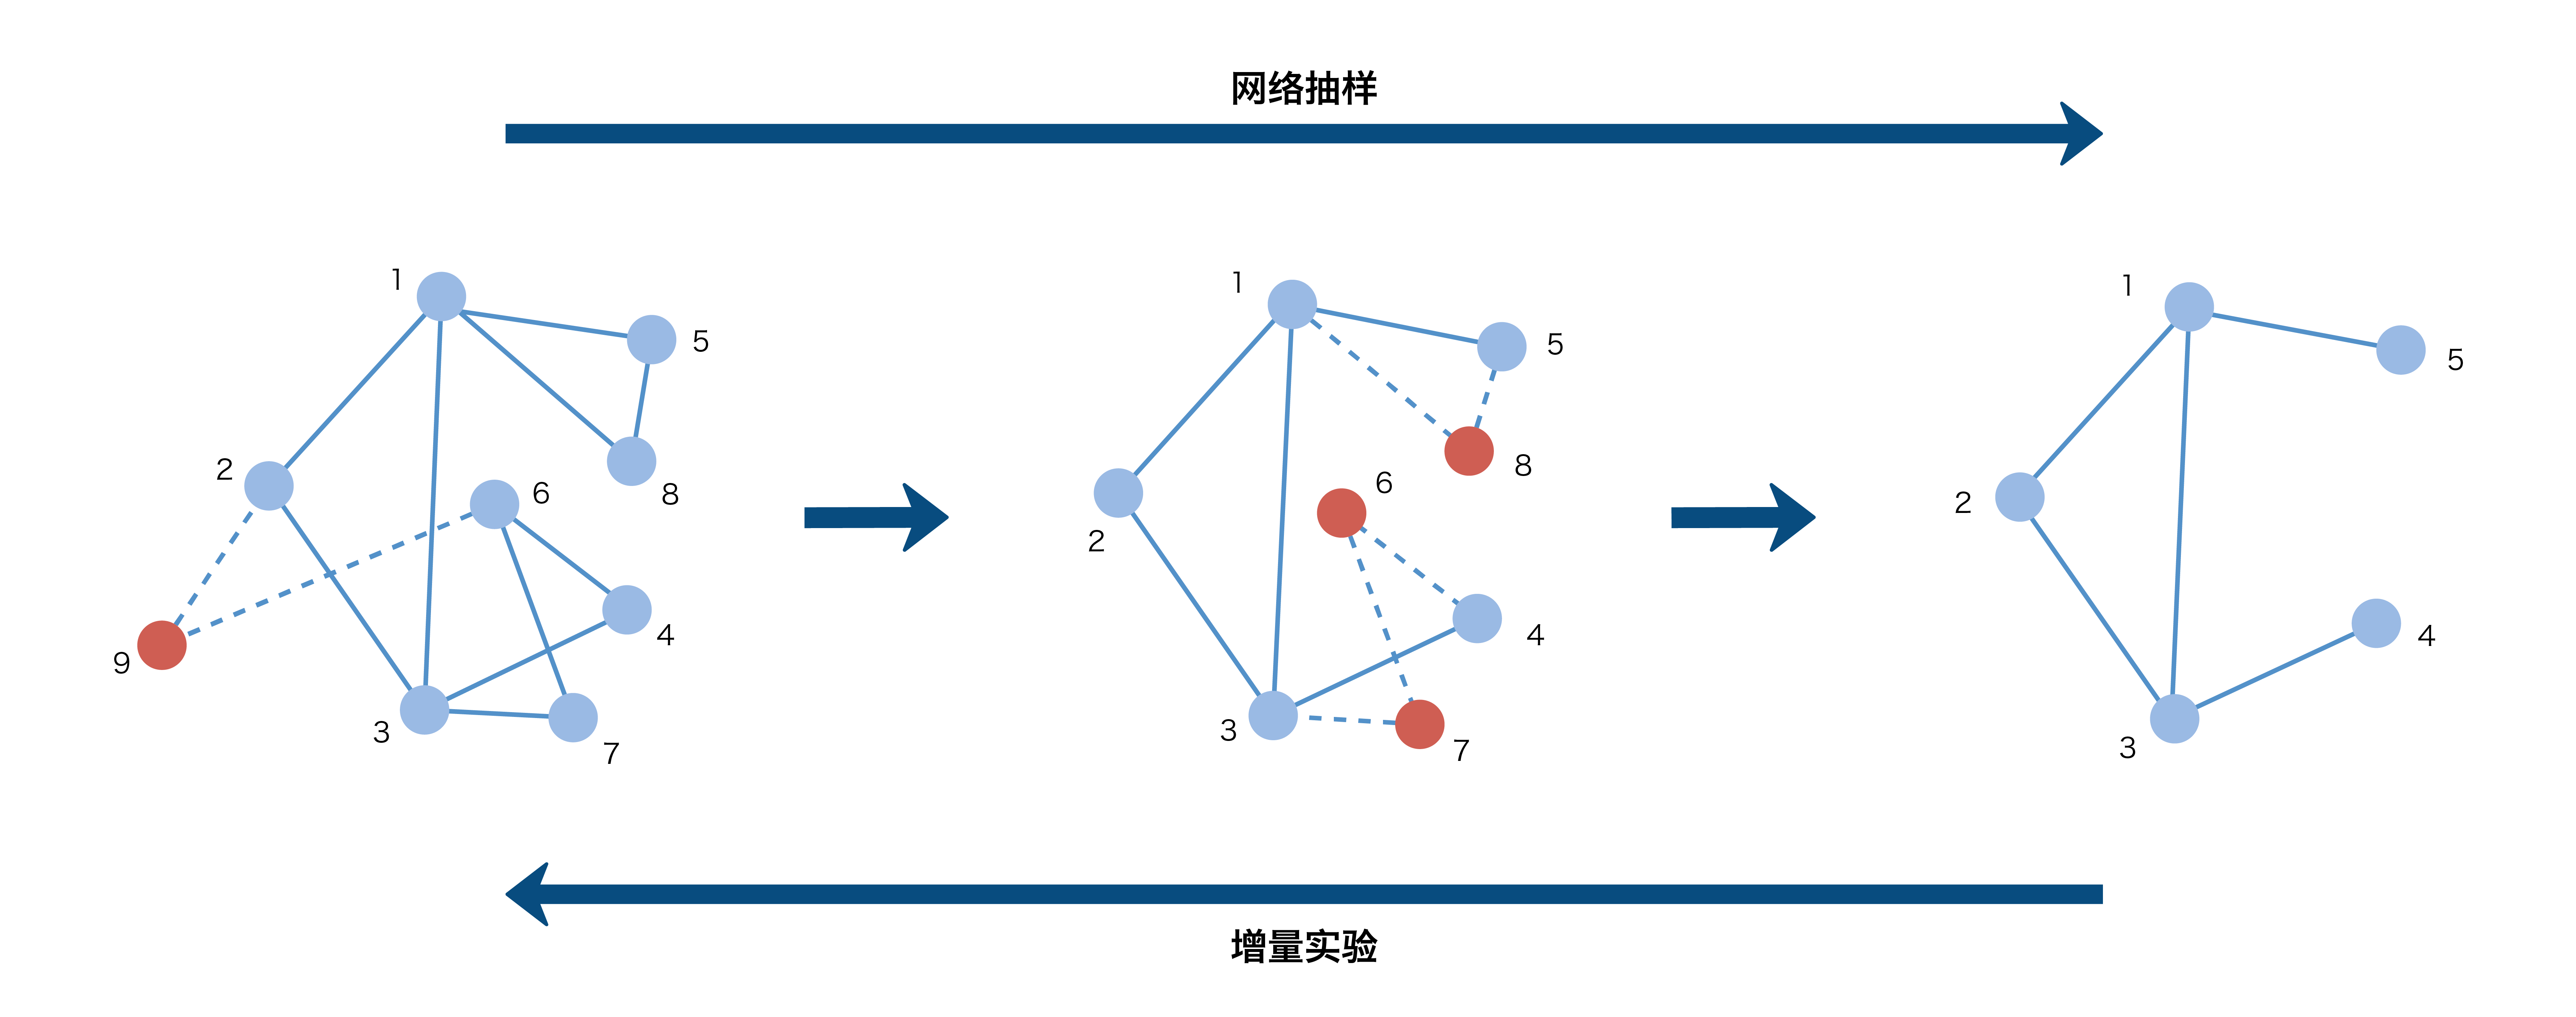
\includegraphics[width=6.2in]{figures/inc_sample}
	\caption{网络采样过程}
\end{figure}


本文研究范围内,在网络的演化过程中,后加入的节点会跟先加入的节点进行连接,否则节点无法在增量场景下进行有效表征,所以增量网络在每个时刻需要保证为全联通图。反之,在抽样过程中,抽样方法需要保证删除节点后剩余子图仍为一个全联通图。在这个基本要求下,随机选取节点进行删除会存在问题,比如下图中如果在某一过程删除了其中的节点5,网络则变成了两个不连通的子图,网络演化过程中的图表征将无法进行。因此在实验中删除节点会根据节点重要性来删除,首先选择删除边缘节点,也即重要性较低的节点,在这一过程中可以通过节点度或节点Pagerank值\cite{page1999pagerank}来对重要性进行衡量,考虑到节点度的局限性,本文实验中采用节点Pagerank值来衡量节点重要性。
\begin{figure}
	\centering
	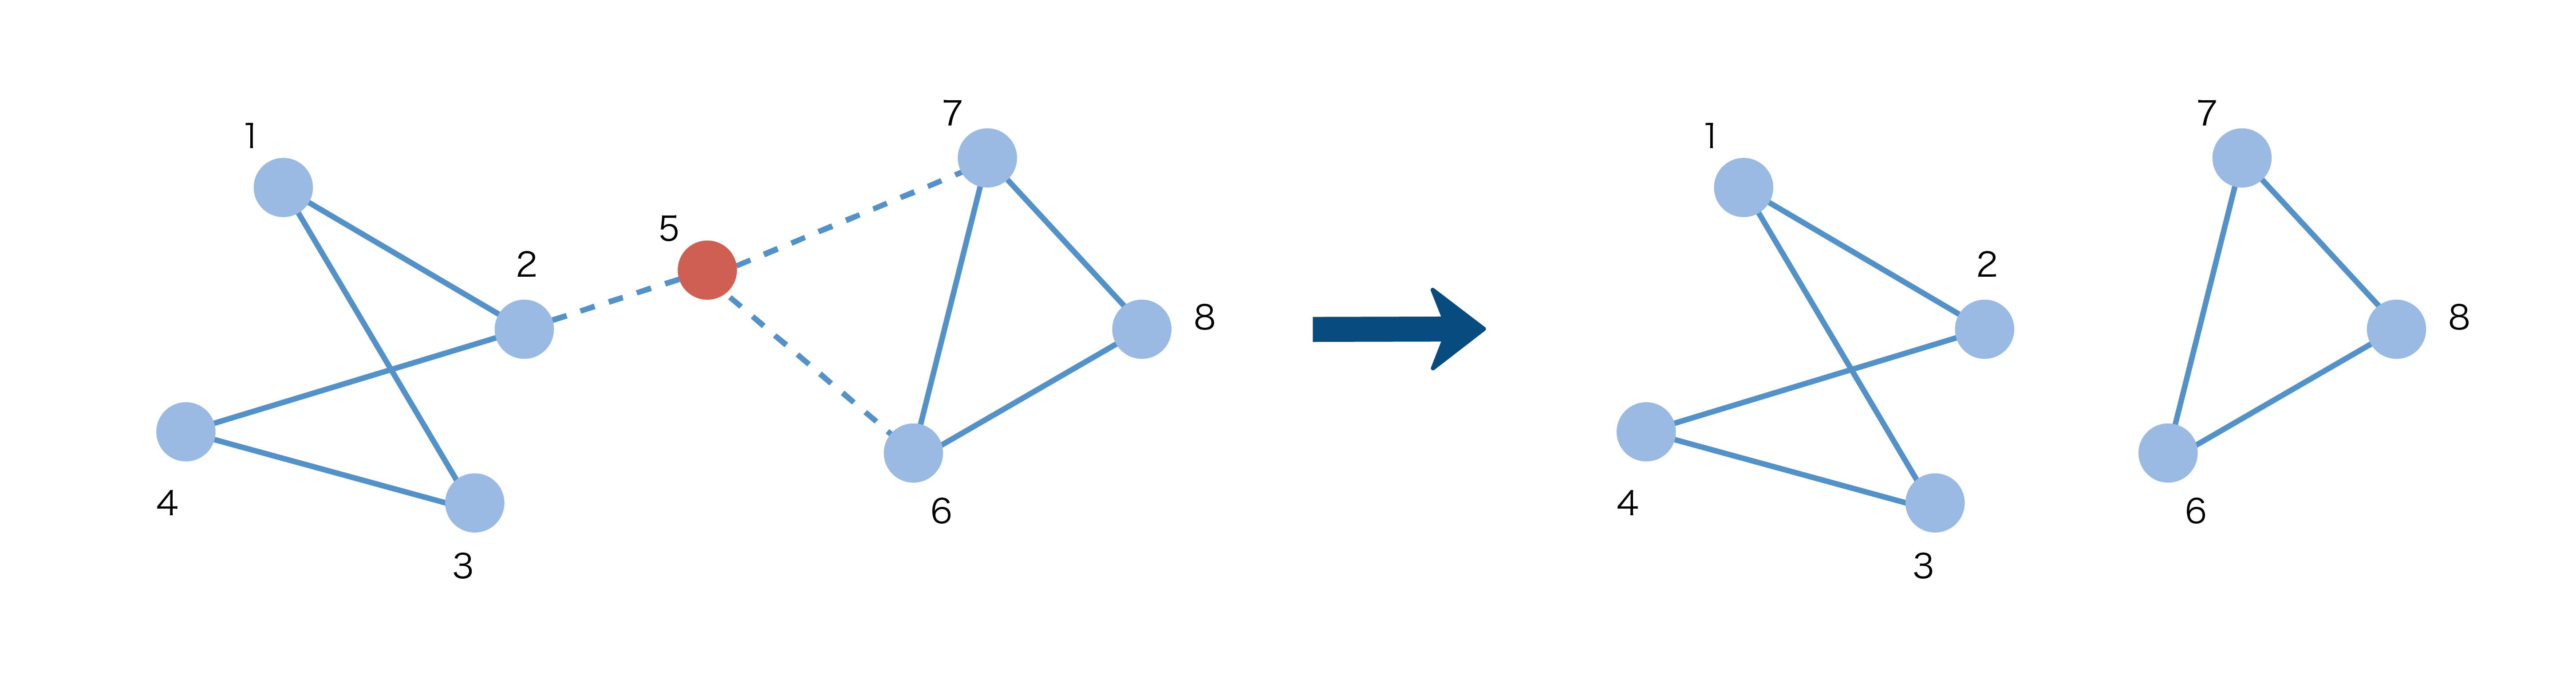
\includegraphics[width=6.2in]{figures/sample_split}
	\caption{随机采样可能出现问题}
\end{figure}


%%%%%%%%%%%%%%%%%%%%%%%%%%%%%%%%%%%%%%%
%----------------------------------------     实验结果与分析     ---------------------------------------%
%%%%%%%%%%%%%%%%%%%%%%%%%%%%%%%%%%%%%%%




%%%%%%%%%%%%%%%%%%%%%%%%%%%%%%%%%%%%%%%
%----------------------------------------     参数设定     ---------------------------------------%
%%%%%%%%%%%%%%%%%%%%%%%%%%%%%%%%%%%%%%%



%%%%%%%%%%%%%%%%%%%%%%%%%%%%%%%%%%%%%%%
%----------------------------------------     实验对比     ---------------------------------------%
%%%%%%%%%%%%%%%%%%%%%%%%%%%%%%%%%%%%%%%
\section{实验对比}
本文提出的TV-LibRec算法充分利用了移动应用间的文本和视图相似性,并以此将功能相近的移动应用聚为一类,进而为开发者推荐第三方库。为了评估本文提出的算法的推荐能力,本文将其与已有的其他著名推荐算法进行比较,从而证明本文提出的算法的有效性。所有对比实验均在本文收集的23,398个移动应用的数据集上进行测试。本文将实验数据集分为两个部分:训练集和测试集,并使测试集占整个数据集的百分比从5\%增加至40\%(步长为5\%),从而比较不同算法在不同比例的测试集下的表现。


\subsection{基准算法}
本文提出的TV-LibRec第三方库推荐算法利用了文本和视图两方面信息,且利用聚类算法将相似移动应用进行聚类,因此在实验比较过程中,将分别对以上算法部分进行实验分析,并与已有的其他著名推荐算法进行比较。具体实验比较将分为以下三分部分:
\begin{itemize}
\item
比较文本与视图相似性。本文提出的TV-LibRec算法中利用了移动应用的文本和视图两个层面的信息,因此本章将分别对这两种相似性进行分析和实验比较。特别的,在文本相似性计算过程中,本文提出了两种计算方法:皮尔森相关系数和余弦相似度,因此也将对这两种相似度计算结果进行比对。

\item
比较不同聚类算法。本文在4.5节中分析和讨论了k-means和单连接的层次聚类算法在移动应用聚类中的优缺点,并提出了本文的k-min聚类算法。为证明聚类算法对第三方库推荐的有效性,本文将使用k-min聚类算法的TV-LibRec,分别与使用k-means、单连接的层次聚类和随机聚类的基准算法进行比较。

\item
与著名推荐算法进行比较。现有推荐算法通常将用户和项目构建成一个用户-项目矩阵(User-Item Matrix),然后对矩阵中的数据进行分析和学习,从而为用户推荐合适的项目。在本文研究问题中,用户为开发者,项目为第三方库。由Salakhutdinov等\cite{salakhutdinov2011probabilistic}提出的概率矩阵分解(PMF: Probabilistic Matrix Factorization)模型,在传统矩阵分解方法的基础上,加入了先验概率,从而能够更准确地为用户推荐项目\cite{liu2013bayesian}。非负矩阵分解(NMF: Non-Negative Matrix Factorization)算法则在传统矩阵分解方法基础上,引入了矩阵中各值非负的规则,从而能够获得更好的推荐效果\cite{luo2014efficient}。此外,本文还将与基于项目的协同过滤算法进行比较(IPCC)\cite{yang2014survey}。
\end{itemize}


\subsection{对比结果与分析}
本文从文本和视图两个层面对移动应用进行相似性计算,其中在文本相似性计算过程中分别使用了皮尔森相关系数和余弦相似度,因此对以上三种相似性计算进行比较。如图5-3所示,其中T-PCC-LibRec表示使用皮尔森相关系数对文本进行相似性计算的第三方库推荐算法,
\begin{figure}
	\centering
	\begin{subfigure}[b]{0.495\textwidth}
		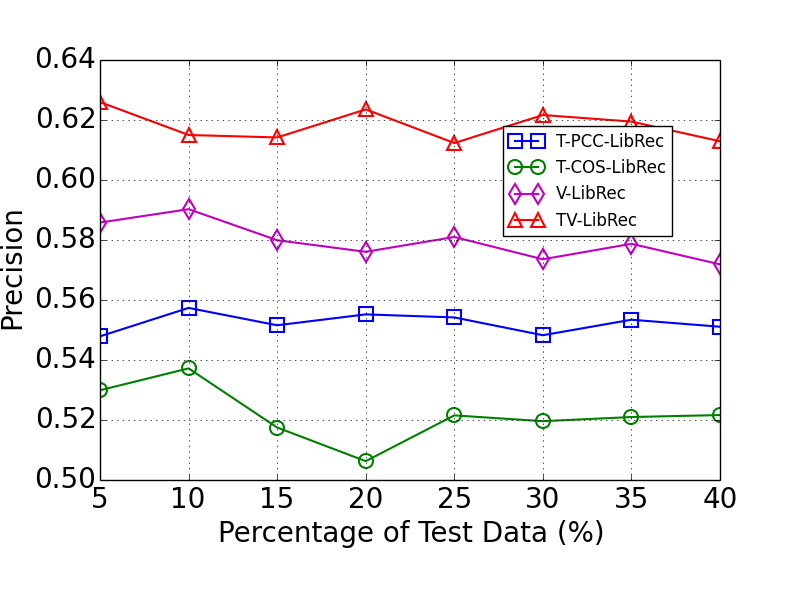
\includegraphics[width=\textwidth]{figures/feature_comp_p}
		\caption{准确率实验结果}
	\end{subfigure}
	\begin{subfigure}[b]{0.495\textwidth}
		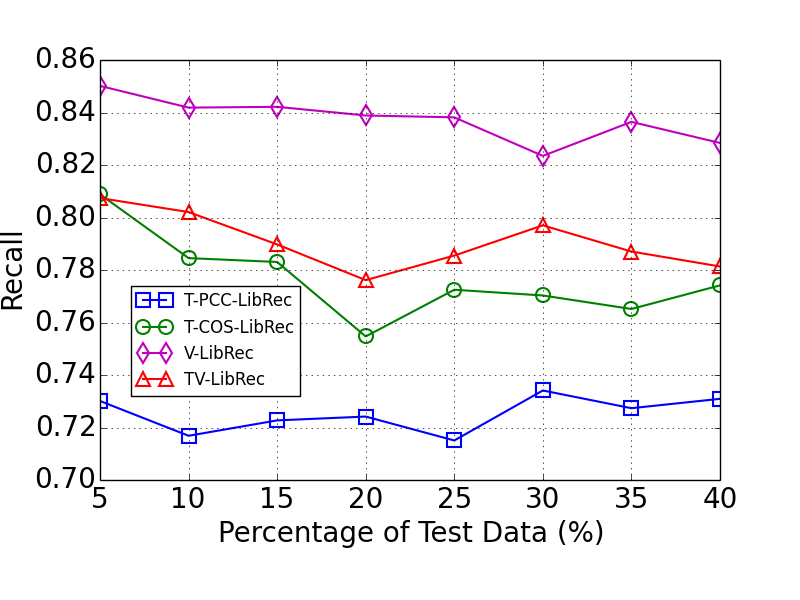
\includegraphics[width=\textwidth]{figures/feature_comp_r}
		\caption{召回率实验结果}
	\end{subfigure}
	\begin{subfigure}[b]{0.5\textwidth}
		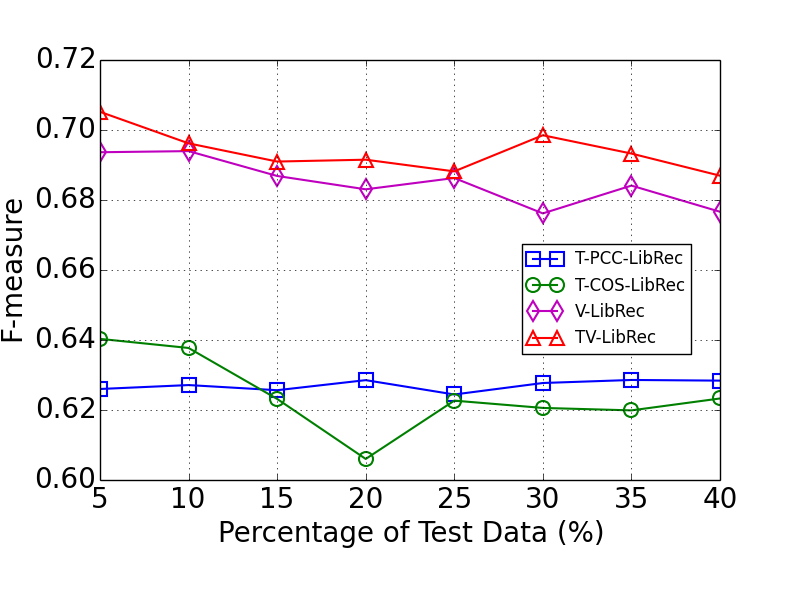
\includegraphics[width=\textwidth]{figures/feature_comp_f}
		\caption{F-measure实验结果}
	\end{subfigure}
	\caption{不同的移动应用特征与相似度计算方法比较。}
\end{figure}
T-COS-LibRec表示使用余弦相似度对文本进行相似性计算的算法,V-LibRec为利用视图相似性的推荐算法,TV-LibRec为同时利用了文本和视图相似性的算法,且使用余弦相似度计算文本间相似性。从图5-3(a)中观察可知,利用移动应用视图层面的相似性能够更准确的为开发者推荐相关第三方库(TV-LibRec和V-LibRec的准确率结果大于T-LibRec),从而说明移动应用代码层相较于描述,包含更多功能信息,更能表征移动应用特征信息。图5-3(b)和5-3(c)同样说明了此问题,证明视图特征在第三方库推荐中优于文本特征。特别的,在图5-3(b)中,V-LibRec的召回率高于TV-LibRec,从侧面说明文本特征反而影响了推荐效果。但综合准确率和召回率,TV-LibRec相比于仅利用文本或视图的推荐算法,具有更好的推荐效果。此外,使用皮尔森相关系数与使用余弦相似度在准确率和召回率上各有优势,从F-measure看,两者的差别并不明显,但余弦相似度在测试集较小的情况下表现优于皮尔森相关系数,现实中更符合这种情况,因此本文选用余弦相似度作为本文相似性计算方法。

本文对相似移动应用进行聚类,以方便搜寻符合开发者需求的相似移动应用。著名的k-means聚类算法和单连接的层次聚类算法能够解决相似移动应用聚类的问题,但其具有一定局限性,因此本文提出了一个更符合移动应用聚类的聚类算法。
\begin{figure}
	\centering
	\begin{subfigure}[b]{0.495\textwidth}
		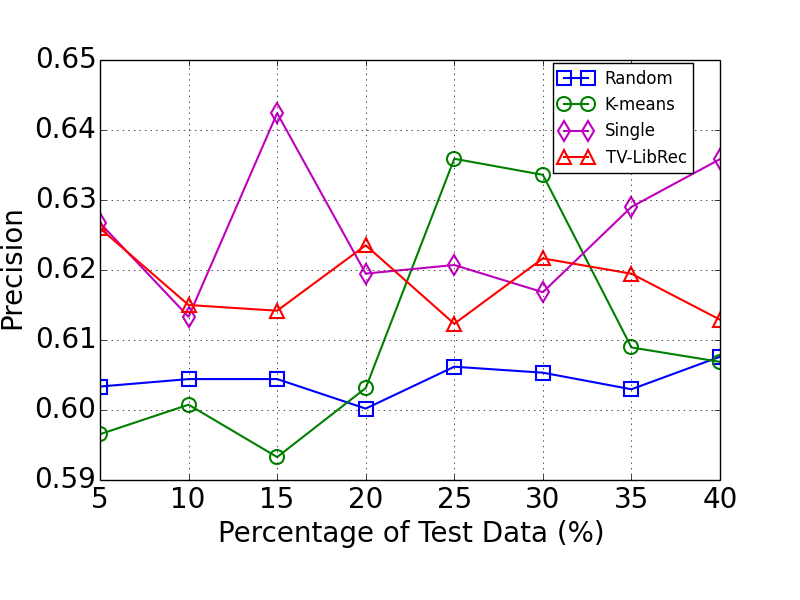
\includegraphics[width=\textwidth]{figures/cluster_comp_p}
		\caption{准确率实验结果}
	\end{subfigure}
	\begin{subfigure}[b]{0.495\textwidth}
		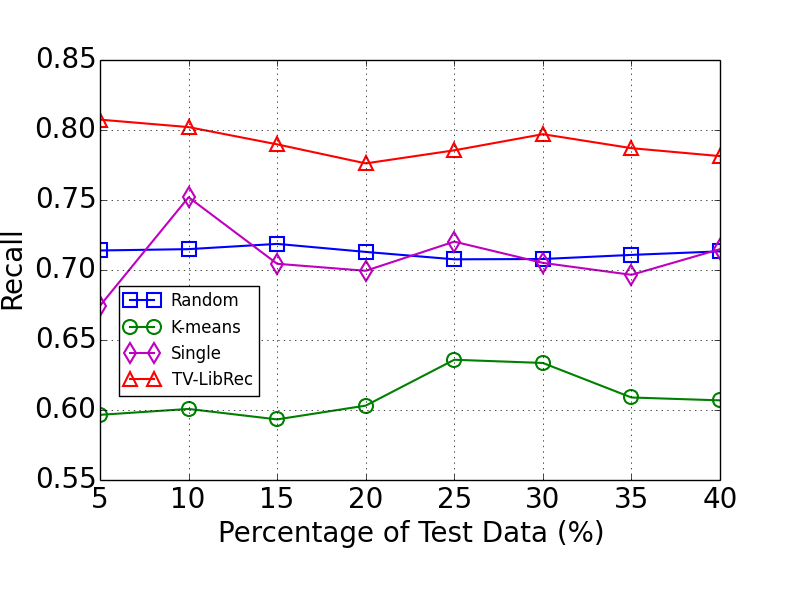
\includegraphics[width=\textwidth]{figures/cluster_comp_r}
		\caption{召回率实验结果}
	\end{subfigure}
	\begin{subfigure}[b]{0.5\textwidth}
		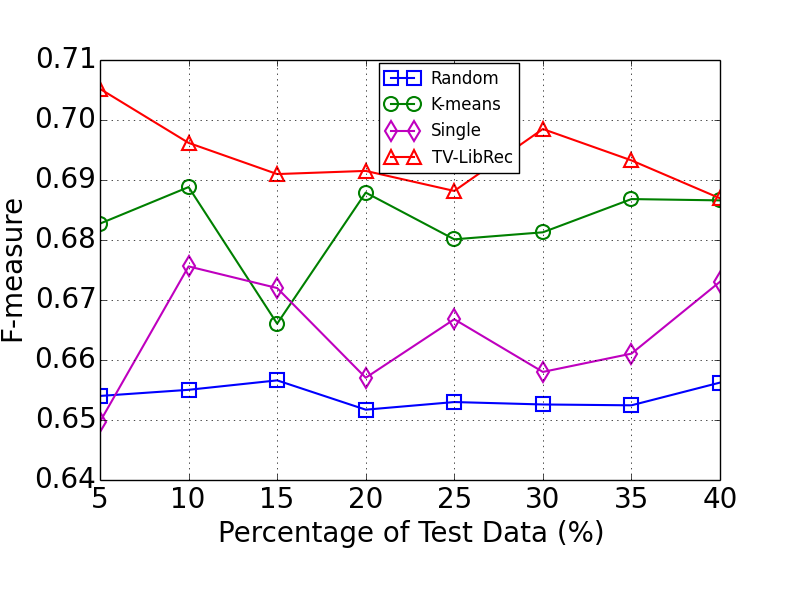
\includegraphics[width=\textwidth]{figures/cluster_comp_f}
		\caption{F-measure实验结果}
	\end{subfigure}
	\caption{不同聚类算法比较。}
\end{figure}
\begin{table*}
\small
\setlength{\tabcolsep}{3.8pt}
\centering
\caption{不同推荐算法的F-measure结果比较}
\begin{tabular}{c c c c c c c c c}
\hline\hline
Test data & 5\% & 10\% & 15\% & 20\% & 25\% & 30\% & 35\% & 40\% \\
\hline
IPCC & 0.061158 & 0.061595 & 0.060085 & 0.059930 & 0.059815 & 0.059352 & 0.059180 & 0.059747 \\

NMF & 0.279595 & 0.272422 & 0.274156 & 0.282729 & 0.293396 & 0.296581 & 0.295678 & 0.296248 \\

PMF & 0.279615 & 0.272791 & 0.281162 & 0.290922 & 0.296766 & 0.296029 & 0.295091 & 0.296159  \\

Random & 0.654009 & 0.655032 & 0.656605 & 0.651721 & 0.652992 & 0.652588 & 0.652447 & 0.656236 \\

TV-LibRec & 0.705193 & 0.696188 & 0.690988 & 0.691516 & 0.688176 & 0.698498 & 0.693270 & 0.686949 \\
\hline\hline
\end{tabular}
\end{table*}
为了验证本文提出的聚类算法的有效性,本文分别与使用k-means聚类算法(K-means)、单连接的层次聚类算法(Single)和不使用任何聚类算法(Random)的推荐方法进行比较,且此三种推荐算法仅是在TV-LibRec的基础上换掉相应的聚类算法,因此仍然利用了移动应用的文本和视图特征。从图5-4(a)中可以观察到,k-means的准确率极为不稳定,大部分结果都低于TV-LibRec,但是有两个实验结果高于TV-LibRec,三个实验结果甚至低于Random。Single的准确率也同样不稳定,有部分结果高于TV-LibRec,但也有部分低于TV-LibRec和k-means。图5-4(b)中的召回率结果相对较为稳定,TV-LibRec要优于其他三种方法,使用k-means聚类的方法召回率不如Random和Single。从综合结果F-measure来看,如图5-4(c)所示,TV-LibRec具有最好的推荐效果,而k-means居其后,单连接的层次聚类算法次之,Random最差。从实验结果可以发现,使用k-means和单连接的层次聚类算法可以达到一定的聚类效果,但正如本文在4.5节中所分析的,这两种方法可能会出现某些非最优的聚类情况,因此在实验中的表现不稳定,且整体效果差于本文提出的k-min聚类算法。

最后,本文与著名的推荐算法IPCC、NMF、PMF进行实验比较,具体实验结果如表5-3所示。从表5-3中观察可知,其中未使用移动应用间的相似性的推荐算法(IPCC、NMF、PMF)结果表现都较差,特别是仅利用了移动应用所使用的第三方库间的相似关系的IPCC。NMF和PMF推荐算法充分利用了整个用户-项目矩阵(移动应用与第三方库构成的矩阵)的全局信息,因此能够更全面的分析开发者所需的功能需求。但由于没有移动应用本身的功能信息,导致这些推荐算法无法有效地从第三方库使用情况中获取功能相关的特征,因此无法给出较好的推荐效果。与之不同的Random方法,虽然未对相似移动应用进行聚类,但是其利用了移动应用在文本和视图层面的特征信息,能够掌握开发者的功能需求,从其他相似移动应用中抽取相应的第三方库,所以其推荐效果会优于前三种方法。TV-LibRec则充分利用了移动应用间的相似性,并对其进行了聚类操作,使得与开发者需求相符的移动应用均在同一簇中,从而能够更好地为开发者推荐所需的第三方库。

根据以上三组对比实验分析可得,本文提出的基于文本和视图的TV-LibRec第三方库推荐算法能够有效地为移动应用开发者推荐第三方库,且优于现有的著名推荐算法,从而说明本文提出的文本和视图特征能够有效地表征移动应用的功能信息和开发者的需求。



%%%%%%%%%%%%%%%%%%%%%%%%%%%%%%%%%%%%%%%
%----------------------------------------     本章小结     ---------------------------------------%
%%%%%%%%%%%%%%%%%%%%%%%%%%%%%%%%%%%%%%%
\section{本章小结}
本章详细介绍了本文所使用的实验数据。该数据是由从Google Play上爬取的23,398个移动应用所组成的,其中包括移动应用的元数据和程序包。元数据一共包括了16类数据,本文在文本特征提取中使用了其中的描述,在第三方库推荐的过程中使用了用户评分,以权衡第三方库的功能和质量关系。对移动应用程序包的分析在本文4.4.1节中做了详细分析和解释,因此本章较为简略地说明了反编译后的数据信息。

为了准确衡量实验结果,本章给出了三种评价标准,分别是准确率、召回率和F-measure。这三种评价标准在推荐系统算法评估中被广泛使用,本文使用同样的评价标准来衡量推荐效果。由于准确率和召回率间常出现矛盾的结论,因此本文着重考虑权衡两者的F-measure评价标准。

对于本文提出的TV-LibRec推荐算法,有5个重要的参数会影响最终的推荐效果。因此,本章对这5个重要参数进行实验分析。在本文的实验数据集上以训练集与测试集9:1的分割方式进行实验,本章确定了每个重要参数在实际实验结果中的最优值,从而作为本文推荐算法的参数设定。

最后,本章将本文提出的TV-LibRec第三方库推荐算法与各基准算法进行比较,从而验证本文算法的有效性。本章一共分成三个部分来研究分析TV-LibRec算法的实验效果:比较TV-LibRec算法中文本和视图特征的有效性;比较TV-LibRec算法中k-min聚类算法的有效性;与其他现有的著名推荐算法进行比较。通过实验分析发现,视图特征相比文本特征,能够更有效地表征移动应用的功能信息,得到了更好的第三方库推荐效果。在文本相似性计算过程中,皮尔森相关系数与余弦相似度两种计算方法并无较大差异,但余弦相似度在较小测试集情况下有较优的表现,符合真实场景,因此作为TV-LibRec中的文本相似性计算方法。本章亦通过实验证明了本文提出的k-min聚类算法在移动应用聚类问题上,比k-means算法和单连接的层次聚类算法有更好更稳定的表现,与本文在4.5节中的分析相符。在与其他著名推荐算法的比较中,TV-LibRec算法表现出了较好的实验结果,且说明了本文提出的移动应用相似性在第三方库推荐中具有重要的作用。